Para analizar los algortimos implementados vamos a utilizar los archivos test1.in y test2.in provistos por la cátedra y realizar una serie de test que nos permitirán en primer caso encontrar parametros buenos con lo que ejecutarlos y posteriormente evaluar el desempeño de la implementación mediante las métricas propuestas por la cátedra.

Dividimos la experimentación en dos secciones, una para cada archivo de prueba. Y evaluaremos los parametros individualmente para cada una de ellas


\subsubsection {Archivo Test1.in}

\subsubsubsection {Algoritmo de K-NN}

Lo primero que vamos a hacer es encontrar un valor de $K$ que nos permita maximizar la cantidad de aciertos, sin tener en consideración las métricas.

Ejecutamos el algoritmos de $K-NN$ variando los valores de k entre {1..20} dejando fija la cantidad de particiones en 10. Luego para cada K nos quedamos con los resultados de la iteración con mas aciertos.

Expresamos los aciertos para cada K en con el siguiente gráfico:



Aca va el grafico.

Como se puede observar la iteración que mas aciertos dió es para $K = 3$. Además se puede observar que a medida que se incrementa el valor de $K$ la cantidad de aciertos va disminuyendo levemente, cumpliendo lo mencionado en la introducción teórica. Cuanto mas corta sea la distancia de los vecinos, mas chances hay de tener un acierto.

Lo siguiente es evaluar fijando el $K$ si el valor de la cantidad de particiones influye en en la cantidad de aciertos. Entonces para eso variamos el número de variamos el número, entre {10..40} incrementando en 10 y tomamos la cantidad de aciertos.

Aca va el grafico.

Como se puede observar la cantidad de particiones no es decisiva a la hora de obtener resultados, ya que no incrementa de forma considerable la cantidad de aciertos. Lo que se observa es que a mayor cantidad de repeticiones, las chances de tener un valor de acierto relativamente mayor se incrementan, esto es solamente debido a que el experimento se repite mas veces y no representa una mejora en la calidad de los resultados.

Caracterizados los valores de $K$ y $Cantidad de Particiones$ que nos dieron mejor cantidad de aciertos. Presentamos las métricas para el mejor caso de cada una de ellas.

Aca iria en forma de tabla y su explicacion


\subsubsubsection {Algoritmo de K-NN con Optimización de PCA}

\subsubsubsection {Algoritmo de K-NN con Optimización de PSL-DA}
Habiendo fijado k = 3 , corremos el test1.in variando el gamma utilizando los valores 1,2,10 y 50. Aqui el grafico
\begin{figure}[H]
\centering
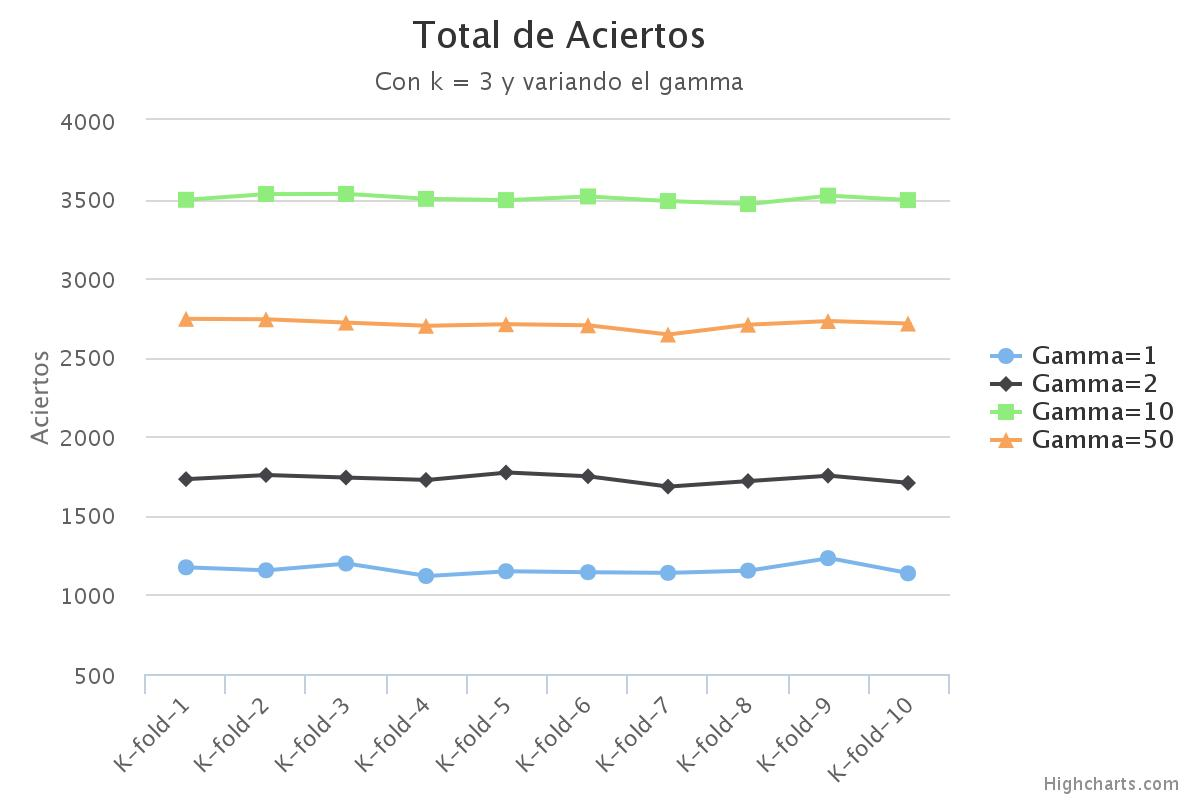
\includegraphics[width=1\textwidth]{chart.jpeg}
\caption{Comparacion de aciertos variando el gamma}
\label{fig:Comparacion de tecnicas}
\end{figure}


Vemos que si aumenta el gamma , mejora la precision pero si gamma aumenta demasiado , en algun momento empeora tu hit rate , suponemos que eso se debe a que si bien tenemos bastante informacion , la cantidad de vecinos no permite aprovecharla . Eso hace suponer que para que tengamos un buen hit rate , debe haber algun tipo de relacion entre el k y el gamma . Eso se va a poner a prueba usando el test2.in

\subsubsection {Archivo Test2.in}

\subsubsubsection {Algoritmo de K-NN}

\subsubsubsection {Algoritmo de K-NN con Optimización de PCA}

\subsubsubsection {Algoritmo de K-NN con Optimización de PSL-DA}

El experimento que nos planteamos es el siguiente. Dejamos fijo el gamma en 13 y hacemos variar el k . Aqui el grafico  
\begin{figure}[H]
\centering
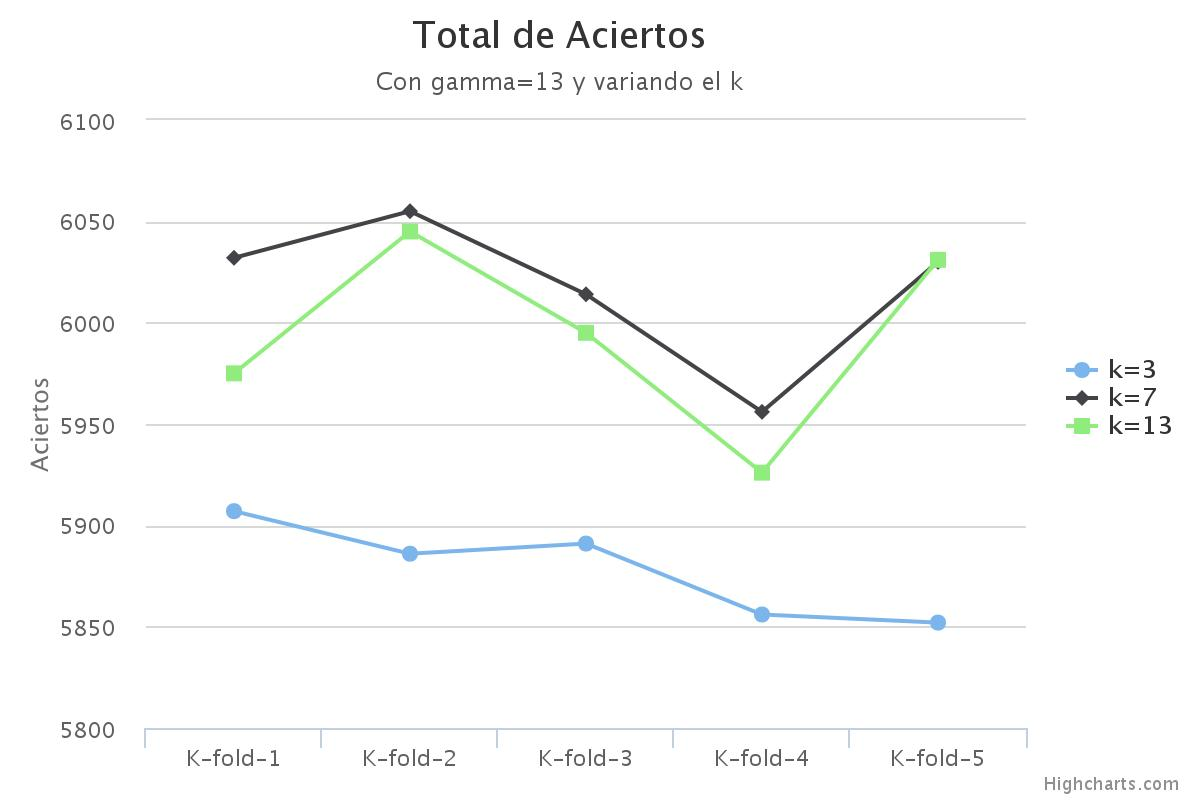
\includegraphics[width=1\textwidth]{chart(2).jpeg}
\caption{Comparacion de aciertos variando el k}
\label{fig:Comparacion de tecnicas}
\end{figure}

De 3 a 7 mejora el hit rate pero es muy poca la mejora en comparacion al aumento de tiempo de computo



